\onslide<1->{
   	\tikzstyle{vertex2} = [opacity = 0]
   	\tikzstyle{vertex3} = [opacity = 0]
    \tikzstyle{vertex4} = [opacity = 0]
   	\tikzstyle{vertex5} = [opacity = 0]
    \tikzstyle{vertex9} = [opacity = 0]
    \tikzstyle{vertex11} = [opacity = 0]
}
\only<2->{\tikzstyle{vertex2} = [opacity = 1]}
\only<3->{\tikzstyle{vertex3} = [opacity = 1]}
\only<4->{\tikzstyle{vertex4} = [opacity = 1]}
\only<5->{
  	\tikzstyle{vertex5} = [opacity = 1]
    \tikzstyle{vertex9} = [opacity = 1]
}

\tikzstyle{end} = [circle, minimum size = 0.6cm, draw = black, inner sep = 0.1pt]
            
\tikzstyle{level 1} = [draw = black, level distance = 1.5cm, sibling distance = 5cm]
\tikzstyle{level 2} = [sibling distance = 2cm]
    
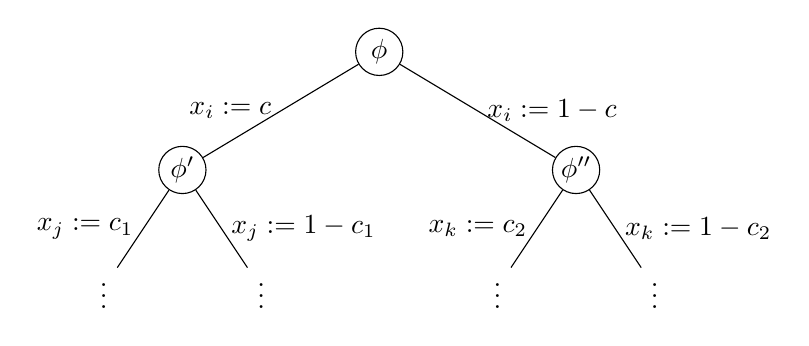
\begin{tikzpicture}[label distance=8mm]
	\node [end] (z){$\phi$}
       	child [vertex2] {node [end] (b) {$\phi'$}
			child [vertex3]{
	           	node {$\vdots$}
                edge from parent
	  	        node[left] {$x_{j} := c_1$}
            }
		    child [vertex4]{
               	node {$\vdots$}
                edge from parent
	   	        node[right] {$x_{j} := 1 - c_1$}
            }
           	edge from parent
            node[left] {$x_{i} := c$}
        }
        child [vertex5] {node [end] (c) {$\phi''$}
           	child [vertex9]{
               	node {$\vdots$}
                edge from parent
	            node[left] {$x_{k} := c_2$}
            }
		    child [vertex9]{
               	node {$\vdots$}
                edge from parent
	            node[right] {$x_{k} := 1 - c_2$}
            }
            edge from parent
	   	    node[right] {$x_{i} := 1 - c$}
        };
\end{tikzpicture}
